\documentclass[a4paper, 12pt]{article}

%%% Работа с русским языком
\usepackage{cmap}					% поиск в PDF
\usepackage{mathtext} 				% русские буквы в формулах
\usepackage[T2A]{fontenc}			% кодировка
\usepackage[utf8]{inputenc}			% кодировка исходного текста
\usepackage[russian]{babel}	% локализация и переносы

%%% Дополнительная работа с математикой
\usepackage{amsmath,amsfonts,amssymb,amsthm,mathtools} % AMS
\usepackage{icomma} % "Умная" запятая: $0,2$ --- число, $0, 2$ --- перечисление

%% Номера формул
%\mathtoolsset{showonlyrefs=true} % Показывать номера только у тех формул, на которые есть \eqref{} в тексте.

%% Шрифты
\usepackage{euscript}	 % Шрифт Евклид
\usepackage{mathrsfs} % Красивый матшрифт

%% Поля
\usepackage[left=2cm,right=2cm,top=2cm,bottom=2cm,bindingoffset=0cm]{geometry}

%% Русские списки
\usepackage{enumitem}
\makeatletter
\AddEnumerateCounter{\asbuk}{\russian@alph}{щ}
\makeatother

%%% Работа с картинками
\usepackage{graphicx}  % Для вставки рисунков
\graphicspath{{images/}{images2/}}  % папки с картинками
\setlength\fboxsep{3pt} % Отступ рамки \fbox{} от рисунка
\setlength\fboxrule{1pt} % Толщина линий рамки \fbox{}
\usepackage{wrapfig} % Обтекание рисунков и таблиц текстом

%%% Работа с таблицами
\usepackage{array,tabularx,tabulary,booktabs} % Дополнительная работа с таблицами
\usepackage{longtable}  % Длинные таблицы
\usepackage{multirow} % Слияние строк в таблице

%% Красная строка
\setlength{\parindent}{2em}

%% Интервалы
\linespread{1}
\usepackage{multirow}

%% TikZ
\usepackage{tikz}
\usetikzlibrary{graphs,graphs.standard}

%% Верхний колонтитул
\usepackage{fancyhdr}
\pagestyle{fancy}

%% Перенос знаков в формулах (по Львовскому)
\newcommand*{\hm}[1]{#1\nobreak\discretionary{}
	{\hbox{$\mathsurround=0pt #1$}}{}}

%% Мои дополнения
\usepackage{float} %Добавляет возможность работы с командой [H] которая улучшает расположение на странице
\usepackage{gensymb} %Красивые градусы
\usepackage{graphicx}               % Импорт изображений
\usepackage{caption} % Пакет для подписей к рисункам, в частности, для работы caption*

% подключаем hyperref (для ссылок внутри  pdf)
\usepackage[unicode, pdftex]{hyperref}

%%% Теоремы
\theoremstyle{plain}                    % Это стиль по умолчанию, его можно не переопределять.
\renewcommand\qedsymbol{$\blacksquare$} % переопределение символа завершения доказательства

\newtheorem{theorem}{Теорема}[section] % Теорема (счетчик по секиям)
\newtheorem{proposition}{Утверждение}[section] % Утверждение (счетчик по секиям)
\newtheorem{definition}{Определение}[section] % Определение (счетчик по секиям)
\newtheorem{corollary}{Следствие}[theorem] % Следстиве (счетчик по теоремам)
\newtheorem{problem}{Задача}[section] % Задача (счетчик по секиям)
\newtheorem*{remark}{Примечание} % Примечание (можно переопределить, как Замечание)
\newtheorem{lemma}{Лемма}[section] % Лемма (счетчик по секиям)

\begin{document}
    \newcommand{\HRule}{\rule{\linewidth}{0.7mm}} % Defines a new command for the horizontal lines, change thickness here
	
	\begin{center}
		\large\textbf{Московский Физико-Технический Институт}\\ % Name of your university/college
		\large\textbf{(государственный университет)}
	
		\vfill
		
		\Large Лабораторная работа по курсу общей физики № *labnum*\\[0.5cm] % Preambule of your document title
		
		
		\HRule
		\\[0.4cm]
		{ \huge \bfseries *name of your labwork*}% Title of your document
		\\[0.4cm] 
		\HRule
		\\[0.5cm]
		
		\ \\
	\textbf{\large Автор:} \\	
	\large *your name* *groupname*\\ % Your name and something more, your group num for example
		\vfill
		\hspace*{-0.8 cm}
\includegraphics[width=100 pt]{frkt_logo}\\ % logo of your  company/university/college
		\large Долгопрудный, 2021 % location and year
	\end{center}

\newpage
\setcounter{page}{2}
\fancyfoot[c]{\thepage}
\fancyhead[L] {Работа № *labnum*} % some information in page header
\fancyhead[R]{}

    \textbf{Цель работы:} исследовать явление дифракции Фринеля и Фраунгофера на щели,
    изучить влияние дифракции наразрешающую способность оптических приборов.

    \textbf{В работе используются:} гелий-неоновый лазер, кассета с набором
    сеток разного периода, щель с микрометрическим винтом, линзы,
    экран, линейка.

    \section{Введение}

    Анализ сложного волнового поля во многих случаях целесообразно проводить, разлагая его на простейшие составляющие, например,
    представляя его в виде разложения по плоским волнам. При этом оказывается, что если мы рассматриваем поле, полученное после прохождения плоской монохроматической волны через предмет или транспарант (изображение предмета на фотоплёнке или стеклянной пластинке)
    с функцией пропускания $t(x)$, то разложение по плоским волнам соответствует преобразованию Фурье от этой функции. Если за предметом
    поставить линзу, то каждая плоская волна сфокусируется в свою точку
    в задней фокальной плоскости линзы. Таким образом, картина, наблюдаемая в фокальной плоскости линзы, даёт нам представление о спектре плоских волн падающего на линзу волнового поля. Поэтому можно
    утверждать, что с помощью линзы в оптике осуществляется пространственное преобразование Фурье.

    \section{Определение ширины щели}
    \subsection{Определение ширины щели по изображению}
    Схема установки представлена на рис. \ref{fig:scheme_I}. Щель переменной ширины $D$, снабжённая микрометрическим винтом $В$, освещается параллельным пучком света, излучаемым лазером. Цена деления винта 10 мкм.
    
    \begin{figure}
    	\centering
    	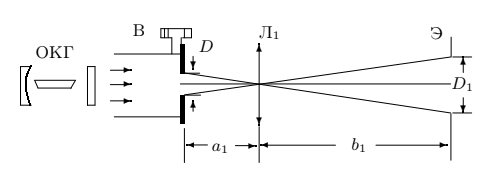
\includegraphics[width=\linewidth]{scheme_I.png}
    	\caption{Схема лабораторной установки для определения ширины щели}
    	\label{fig:scheme_I}
    \end{figure}

	Увеличенное изображение щели с помощью линзы Л1 проецируется на экран Э. Величина изображения $D_1$ зависит от расстояний от линзы до предмета -- $a_1$ и до изображения — $b_1$, т. е. от увеличения $\Gamma$ системы:
	
	\begin{equation}
		\Gamma=\frac{D_{1}}{D}=\frac{b_{1}}{a_{1}}
	\end{equation}
	
	Снимем зависимость ширины изображения щели $D_1$ от $D$, результаты занесем в таблицу \ref{table:table_1}.
	
	\begin{table}[]
    \centering
    \begin{tabular}{|c|c|}
        \hline
        $D$, мкм & $D_1$ мм \\ \hline
        50       & 2         \\ \hline
        100      & 4         \\ \hline
        150      & 6         \\ \hline
        200      & 7         \\ \hline
        250      & 8         \\ \hline
        300      & 10        \\ \hline
        350      & 12        \\ \hline
        400      & 13        \\ \hline
        450      & 14        \\ \hline
        500      & 15        \\ \hline
    \end{tabular}
	\caption{Таблица эксперементальных данных -- зависимость $D_1(D)$}
	\label{table:table_1}
\end{table}
	
	\begin{center}
		$F = 43$ мм -- фокусное расстояние линзы Л1 \\
		$L = 1339$ мм -- расстояние от щели до экрана \\
		$a_1 = 50$ мм -- расстояние от щели до линзы \\
		$b_1 = 1289$ мм -- расстояние от линзы до экрана \\
		$D_0 = 630$ мкм -- начало отсчета ширины щели \\
	\end{center}

	Используя измеренные величины $a_1$ и $b_1$ найдем увеличение линзы
	\[ \Gamma = \frac{b_1}{a_1} = 25.78 \]

	Решая уравнение
	\[ \frac{1}{a_1} + \frac{1}{L - a_1} = \frac{1}{F} \]
	получаем $a_1 \approx 44.48$ мм, откуда $b_1 \approx$ мм. Таким образом, можем найти увеличение линзы
	\[ \Gamma = \frac{L - a_1}{a_1} \approx 29.1 \]
    
    По эксперементальным данным построим график зависимости $D_1(D)$, по наклону графика и пересечению его с осью Ox определим увеличение линзы.
    
    \begin{figure}
    	\centering
    	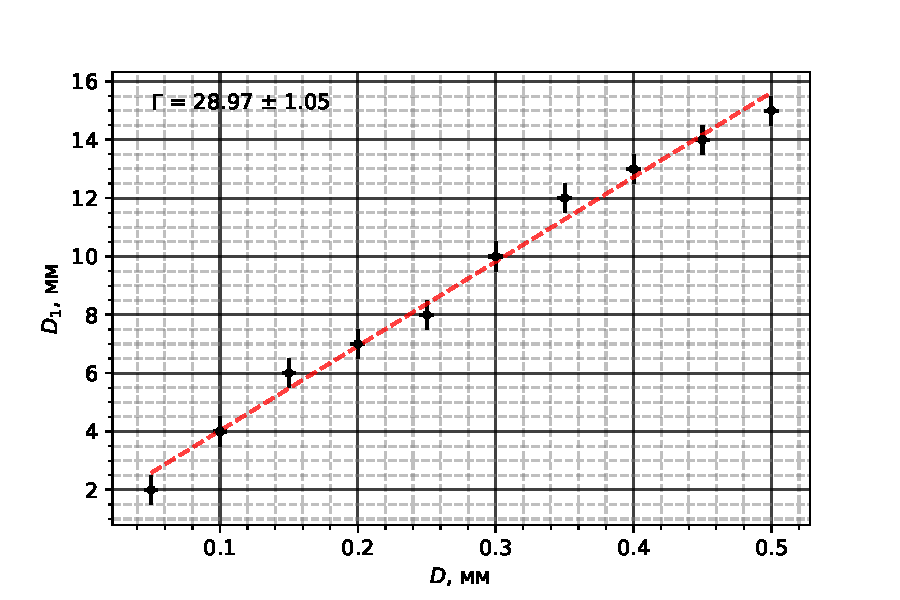
\includegraphics[width=\linewidth]{D_D1.pdf}
    	\caption{Зависимость $D1(D)$}
    \end{figure}

	Увеличение линзы $\Gamma = 28,97$.
    
    \subsection{Определение ширины щели по спектру}
    
    Убрав линзу, можем наблюдать на экране спектр светового луча после прохождения через щель.
    
    \begin{figure}
    	\centering
    	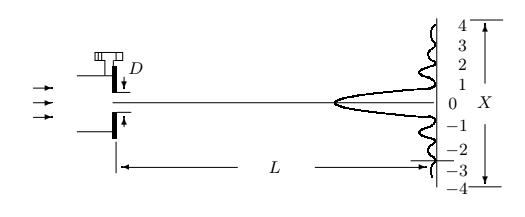
\includegraphics[width=\linewidth]{scheme_II.png}
    	\caption{Спектр щели}
    	%\label{key}
    \end{figure}

	Изменяя ширину щели измерим расстояние между m-ми максимумами спектрального разложения. Результаты представлены в таблице \ref{table:DsSpectr}.
	
	\begin{table}[h!]
    \centering
    \begin{tabular}{|c|c|c|c|c|}
    \hline
    $D$, мкм  & $X$, мм  & m  & $Ds$, мм   & $\sigma_{D_s}$, мм   \\ \hline
    50        & 85       & 2  & 0,04       & 0,0002               \\ \hline
    100       & 53       & 2  & 0,06       & 0,0006               \\ \hline
    150       & 56       & 4  & 0,12       & 0,0011               \\ \hline
    200       & 55       & 6  & 0,19       & 0,0017               \\ \hline
    250       & 66       & 10 & 0,26       & 0,0019               \\ \hline
    300       & 39       & 8  & 0,35       & 0,0045               \\ \hline
    350       & 47       & 10 & 0,36       & 0,0038               \\ \hline
    400       & 42       & 10 & 0,40       & 0,0048               \\ \hline
    450       & 35       & 8  & 0,39       & 0,0055               \\ \hline
    \end{tabular}
    \caption{}
    \label{table:DsSpectr}
\end{table}
	
	По результатам эксперемента вычислим ширину щели, используя соотношение
	
	\begin{equation}
		\Delta X = \frac{X}{2 m} = \frac{\lambda}{D_s} L
	\end{equation}
	где $L = 1342$ мм -- расстояние от щели до экрана, а $lambda$ -- длина волны. Длина волны лазера He-Ne $\lambda = 632.8$ нм.

    \section{Определение периода сеток}
    \subsection{Определение периода сеток по спектру}
    
    Поставим кассету с двумерными решётками (сетками) вплотную к выходному окну лазера. Для каждой сетки измерим расстояние $X$ между $m$-ми пиками и отметим $m$ -- количество пиков. Рассчитаем расстояния $\Delta X$ между соседними максимумами и определим период каждой решётки $d$, используя соотношения:
    
    \begin{equation}
    \Delta X=\frac{X}{m}=\frac{\lambda}{d} L
    \end{equation}
    где $L = 1317$ мм -- расстояние от касеты до экрана. Результаты занесем в таблицу \ref{table:difraction}.
    
	\begin{minipage}{0.4\textwidth}
		\centering
		\begin{tabular}{|c|c|c|c|}
			\hline
			Решетка    & $X$, мм  & $m$ & $d$, мм \\ \hline
			1          & 147      & 2   & 0.02    \\ \hline
			2          & 99       & 2   & 0.03    \\ \hline
			3          & 50       & 2   & 0.07    \\ \hline
			4          & 37       & 3   & 0.14    \\ \hline
			5          & 28       & 3   & 0.18    \\ \hline
		\end{tabular}
		\captionof{table}{Дифракция без линзы}
		\label{table:difraction}
	\end{minipage}
	\begin{minipage}{0.4\textwidth}
		\centering
		\begin{tabular}{|c|c|c|c|}
			\hline
			Решетка    & $X$, мм   & $m$ & $d$, мм \\ \hline
			2          & 210       & 1   & 0.03    \\ \hline
			3          & 104       & 1   & 0.06    \\ \hline
			4          & 105       & 2   & 0.12    \\ \hline
			5          & 79        & 2   & 0.16    \\ \hline
		\end{tabular}
		\captionof{table}{Дифракция с линзой}
		\label{table:lense_difractiton}
	\end{minipage}
    
    \begin{figure}
    	\centering
    	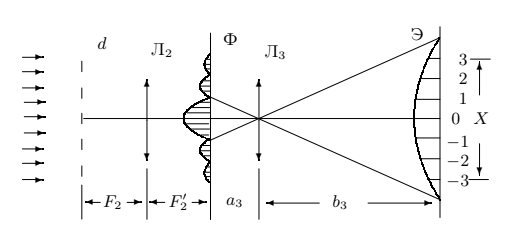
\includegraphics[width=\linewidth]{scheme_III.png}
    	\caption{text}
    	%\label{key}
    \end{figure}
    
    \subsection{Определение периода сеток по увеличенному изображению спектра}
    
    Далее линзу Л2 с максимальным фокусом $(F_2 = 110$ мм поставим на расстоянии $\simeq F_{2}$ от кассеты. В плоскости Ф линза Л2 даёт Фурье-образ -- сетки её спектр, а короткофокусная линза Л3 ($F_3 = 25$ мм) создаёт на экране увеличенное изображение этого спектра.
    Измерим $X$ и $m$ для всех сеток, где это возможно. Так как экран достаточно удалён $\left(b_{3} \gg a_{3}\right)$, то практически $a_{3}=F_{3}$, и расстояние между линзами $\simeq F_{2}+F_{3}$. Результаты измерений представлены в таблице \ref{table:lense_difractiton}.

	Вычислим увеличение линзы Л3: $\Gamma_3 = \frac{b_3}{a_3}$. $a_3 \approx F_3$, из геометрических соображений очевидно, что $b_3 = L - F_3 - 2F_1$. Тогда $b_3 = 1072$ мм, откуда $\Gamma_3 = 42.88$.
	
	Тогда для нахождения периода сетки воспользуемся соотношением
	
	\begin{equation}
		\frac{\Delta X}{\Gamma_3} = \frac{\lambda}{d} F_2
	\end{equation}
	
	откуда
	
	\[ d = \frac{2 m \lambda \Gamma_3 F_2}{X} \]

    \section{Исследование мультиплицированного изображения щели}
    
    Снова поставим тубус со щелью к окну лазера и найдем на экране резкое изображение щели с помощью линзы Л2 ($F_2 = 110$ мм). В фокальной плоскости $\Phi$ линзы Л2 поставим кассету с сетками, которые будут <<рассекать>> Фурье-образ щели -- осуществлять пространственную фильтрацию.
    
    Снимем зависимость $Y$ (расстояние между удалёнными изображениями щели и и $K$ (число промежутков между изображениями) от $n$ (номер сетки) для фиксированной ширины входной щели. Данные занесем в таблицу \ref{table:multiplication}.
    
    \begin{table}[h!]
    \centering
    \begin{tabular}{|c|c|c|c|c|}
    \hline
    Решетка    & $Y$, мм & $K$ & $\Delta y$, мм & $\sigma_{\Delta y}$, мм \\ \hline
    1          & 102     & 4   & 3.58           & 0.010                   \\ \hline
    2          & 72      & 4   & 2.53           & 0.007                   \\ \hline
    3          & 36      & 4   & 1.26           & 0.004                   \\ \hline
    4          & 27      & 6   & 0.63           & 0.002                   \\ \hline
    5          & 21      & 6   & 0.49           & 0.002                   \\ \hline
    \end{tabular}
    \caption{Мультиплицирование}
    \label{table:multiplication}
\end{table}
    
    \begin{figure}
    	\centering
    	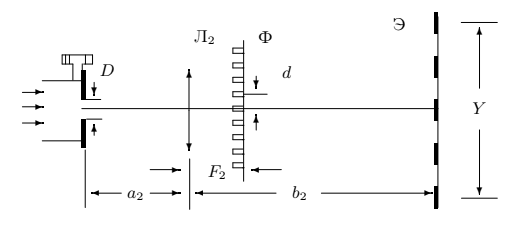
\includegraphics[width=\linewidth]{scheme_IV.png}
    	\caption{Мультиплицирование}
    	%\label{key}
    \end{figure}

	\begin{center}
		$L = 1339$ мм -- расстояние от щели до экрана \\
		$a_2 = 165$ мм -- расстояние от щели до линзы \\
		$b_2 = 1174$ мм -- расстояние от линзы до экрана \\
		$F_2 = 110$ мм --фокусное расстояние линзы \\
		$D = 340$ мм -- ширина щели
	\end{center}

	Увеличение линзы $\Gamma_2 \approx 7.12$. Рассчитаем периоды $\Delta y$ <<фиктивных>> решёток, которые дали бы такую же периодичность на экране: $\Delta y=\Delta Y / \Gamma_{2}$, где $\Delta Y=Y / K .$ Результаты представлены в таблице \ref{table:multiplication}.
	
	Построим график зависимости $\Delta y(\frac{1}{d})$, где $d$ -- период решетки, определенный по спектру. Зависимость должна быть линейной, поскольку
	
	\begin{equation}
		\Delta y = \lambda F_2 \frac{1}{d}
	\end{equation} 
	
	\begin{table}[]
    \centering
    \begin{tabular}{|c|c|c|c|c|c|}
    \hline
    $\Delta y$, мм & 3,58 & 2,53 & 1,26 & 0,63 & 0,49 \\ \hline
    $d$, мм        & 0,02 & 0,03 & 0,07 & 0,14 & 0,18 \\ \hline
    \end{tabular}
\end{table}
	
	\begin{figure}
		\centering
		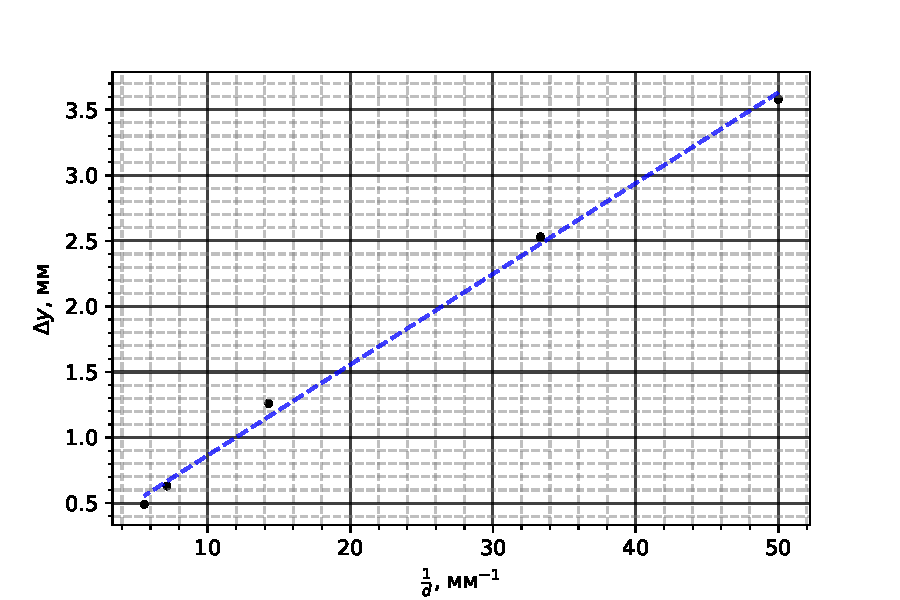
\includegraphics[width=\linewidth]{Delta_y_d.pdf}
		\caption{график зависимости $\Delta y(\frac{1}{d})$}
	\end{figure}

	\section{Вывод}

    
\end{document}